\section{Transmitter Blokken}

\subsection{Action (Kristian T.)}

\begin{figure}[h]
\centering
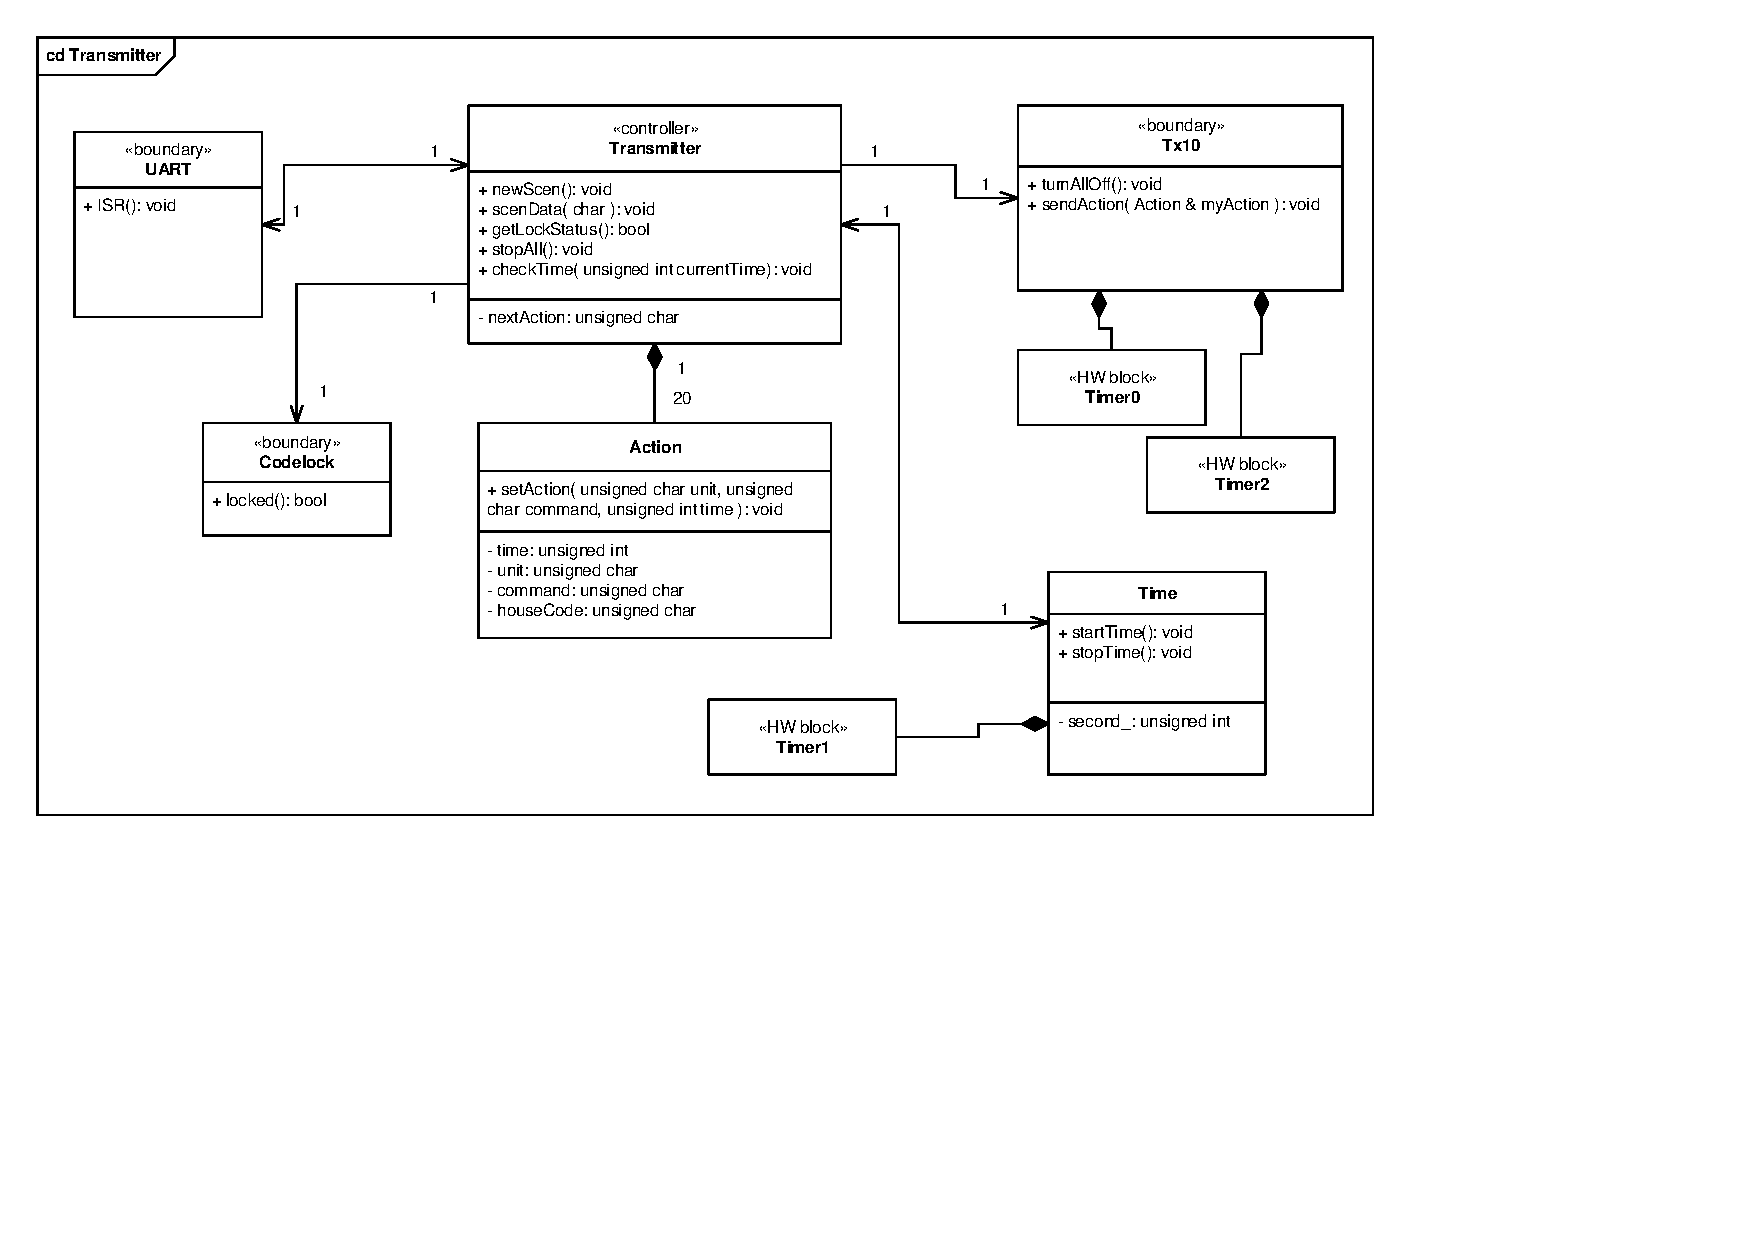
\includegraphics[scale=1,clip=true, trim=210 288 442.4 203]{Systemarkitektur/diagrammer/Transmitter_Klassediagram} %L B R T - HUSKE DET
\end{figure}

%setAction
\begin{table}[h]
\begin{tabularx}{\textwidth}{p{0.6 cm} l X} %\hline
\multicolumn{3}{l}{\textbf{setAction}}\\
& Operation: & %Skriv tekst herunder
\texttt{void setAction( unsigned char unit, unsigned char command, unsigned int time ) }
\\ & Parametre: & %Skriv tekst herunder
Modtager enhed, kommando og tidspunkt relativt til starttidspunktet for aktionen.
\\ & Returværdi: & %Skriv tekst herunder
-
\\ & Beskrivelse: & %Skriv tekst herunder
Metodens formål er primært at gemme informationer i en aktion. Metoden skal selv sætte houseCode baseret på hvilken enhed, den kaldes med. De forskellige houseCode værdier kan ses nedenfor:

Lamper: 1

TV: 2

Radio: 3
\\ \end{tabularx}
\end{table}


%attributter
\begin{table}[h]
\centering
\begin{tabularx}{13 cm}{|l |X|} \hline
Attribut & Beskrivelse \\ \hline

\texttt{unsigned int time} & Gemmer tiden i minutter for den pågældende aktion relativt til det tidspunkt scenariet sættes igang. \\ \hline
\texttt{unsigned char unit} & Gemmer hvilken enhed, aktionen skal gælde for. \\ \hline
\texttt{unsigned char command} & Gemmer hvilken kommando, aktionen skal sende. \\ \hline
\texttt{unsigned char houseCode} & Gemmer huskoden, for den enhed der skal manipuleres. \\ \hline
\end{tabularx}
\end{table}

\clearpage
\subsection{Codelock (David)}

\begin{figure}[h]
\centering
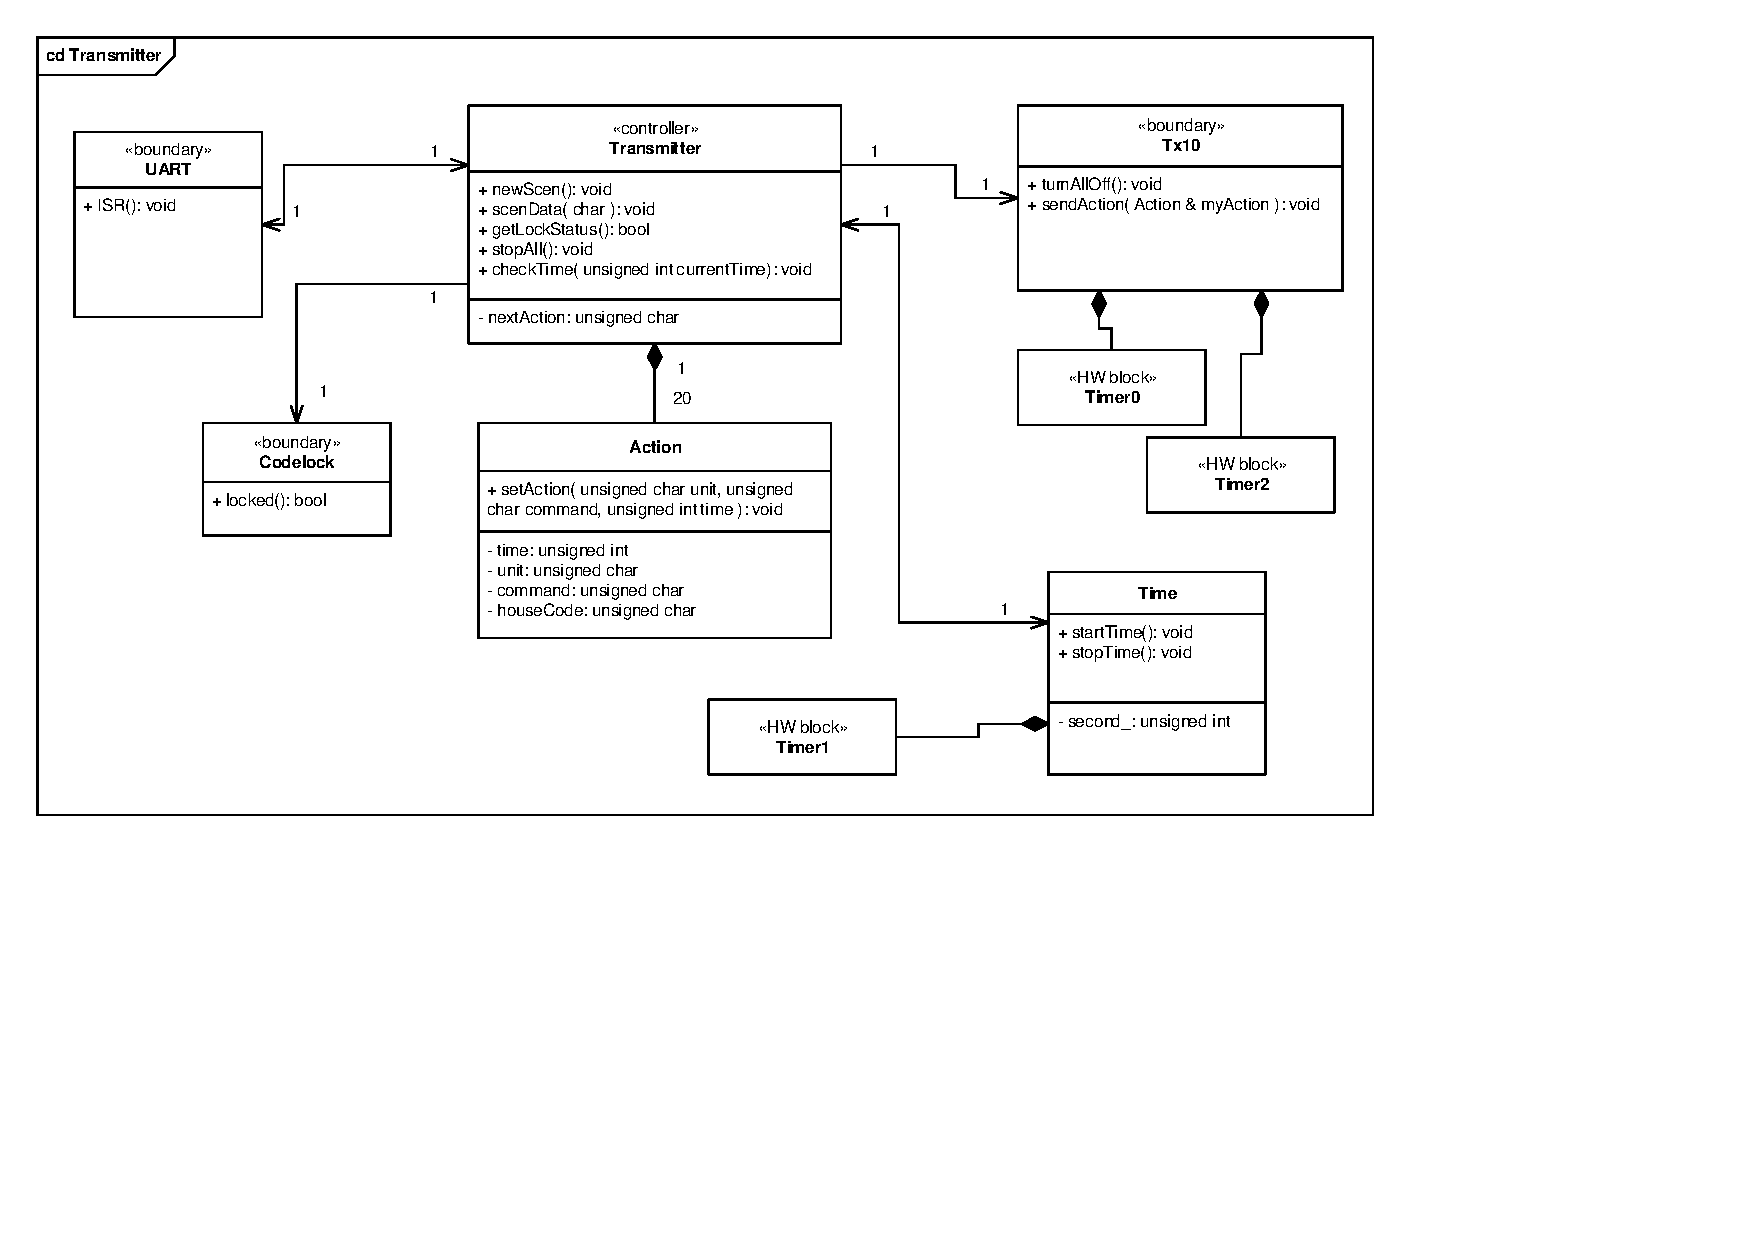
\includegraphics[scale=1,clip=true, trim=80 330 650 203]{Systemarkitektur/diagrammer/Transmitter_Klassediagram} %L B R T - HUSKE DET
\end{figure}

\begin{table}[h]
\begin{tabularx}{\textwidth}{p{0.6 cm} l X} %\hline
\multicolumn{3}{l}{\textbf{unlocked}}\\
& Operation: & %Skriv tekst herunder
\texttt{bool unlocked( void )}
\\ & Parametre: & %Skriv tekst herunder
ingen parametre
\\ & Returværdi: & %Skriv tekst herunder
\texttt{TRUE} hvis den er åben. \texttt{FALSE} hvis den ikke er åben.
\\ & Beskrivelse: & %Skriv tekst herunder
Tjekker om koden er tastet rigtigt ind på vores DE2 board.
\\ \end{tabularx}
\end{table}

\subsection{Time (Kasper)}

\begin{figure}[h]
\centering
\includegraphics[scale=1,clip=true, trim=503 213 230 275]{Systemarkitektur/diagrammer/Transmitter_KlasseDiagram} %L B R T - HUSKE DET
\end{figure}

\begin{table}[h]
\begin{tabularx}{\textwidth}{p{0.6 cm} l X} %\hline
\multicolumn{3}{l}{\textbf{Time}}\\
& Operation: & %Skriv tekst herunder
\texttt{Void Time( )}
\\ & Parametre: & %Skriv tekst herunder
-
\\ & Returværdi: & %Skriv tekst herunder
- 
\\ & Beskrivelse: & %Skriv tekst herunder
-initialisere timer 1 til at interupt hvert sekund.
\\ \end{tabularx}
\end{table}

\clearpage

\begin{table}[h]
\begin{tabularx}{\textwidth}{p{0.6 cm} l X} %\hline
\multicolumn{3}{l}{\textbf{startTime}}\\
& Operation: & %Skriv tekst herunder
\texttt{Void startTime ( void )}
\\ & Parametre: & %Skriv tekst herunder
-
\\ & Returværdi: & %Skriv tekst herunder
- 
\\ & Beskrivelse: & %Skriv tekst herunder
-starter tidstælling på timeren. Tiden tælles op hvert minut.
\\ \end{tabularx}
\end{table}

\begin{table}[h]
\begin{tabularx}{\textwidth}{p{0.6 cm} l X} %\hline
\multicolumn{3}{l}{\textbf{stopTime}}\\
& Operation: & %Skriv tekst herunder
\texttt{Void stopTime ( void )}
\\ & Parametre: & %Skriv tekst herunder
-
\\ & Returværdi: & %Skriv tekst herunder
- 
\\ & Beskrivelse: & %Skriv tekst herunder
-stopper tidstælling på timeren.
\\ \end{tabularx}
\end{table}


\begin{table}[h]
\begin{tabularx}{\textwidth}{p{0.6 cm} l X} %\hline
\multicolumn{3}{l}{\textbf{operator++}}\\
& Operation: & %Skriv tekst herunder
\texttt{operator++()}
\\ & Parametre: & %Skriv tekst herunder
-
\\ & Returværdi: & %Skriv tekst herunder
- 
\\ & Beskrivelse: & %Skriv tekst herunder
-inkremere atributten second med 1.
\\ \end{tabularx}
\end{table}

\begin{table}[h]
\centering
\begin{tabularx}{13 cm}{|l |X|} \hline
Attribut & Beskrivelse \\ \hline
unsigned int second & indeholder tiden i sekunder. \\ \hline
\end{tabularx}
\end{table}

\clearpage

\subsection{Transmitter (Kristian S.)}

\begin{figure}[h]
\centering
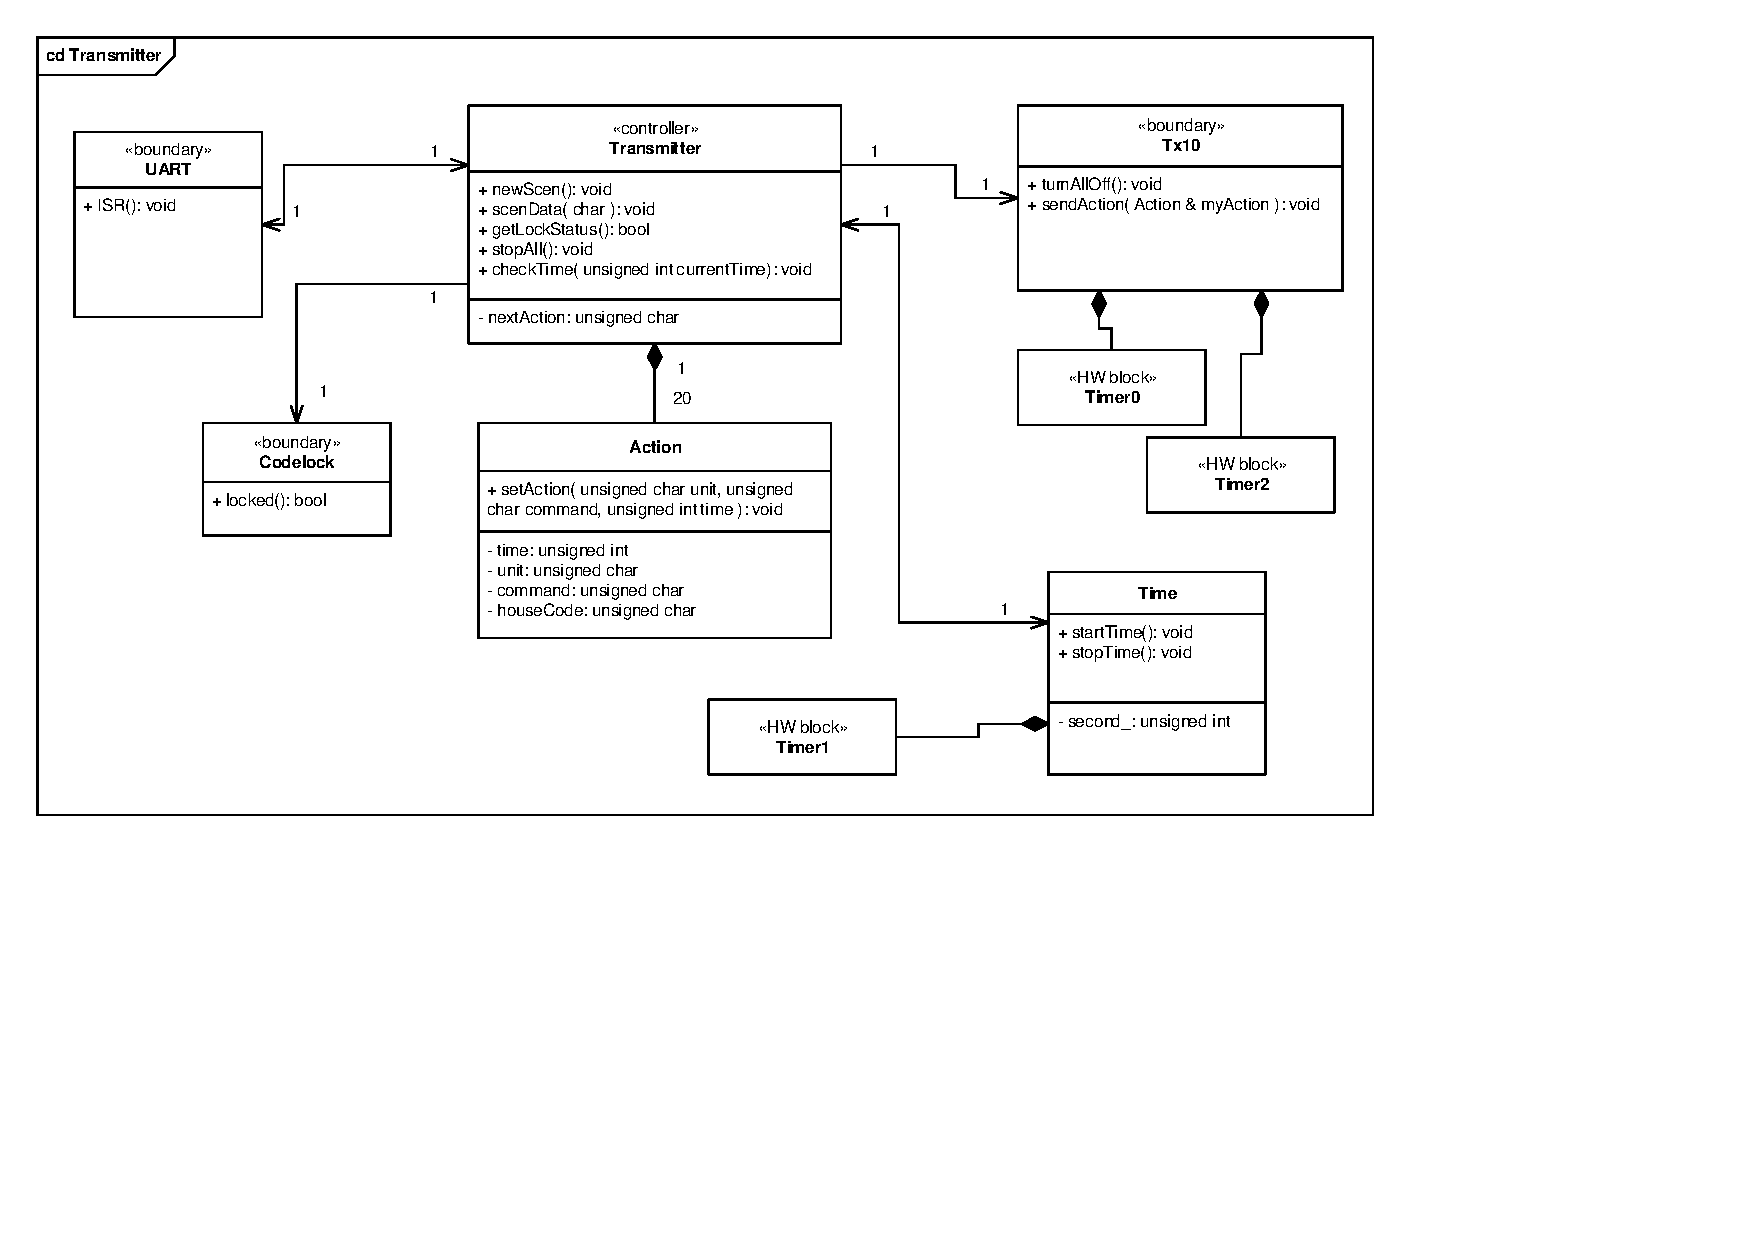
\includegraphics[scale=1,clip=true, trim=225 429 437 50]{Systemarkitektur/diagrammer/Transmitter_Klassediagram} %L B R T - HUSKE DET
\end{figure}

\begin{table}[h]
\begin{tabularx}{\textwidth}{p{0.6 cm} l X} %\hline
\multicolumn{3}{l}{\textbf{\texttt{newScen}}}\\
& Operation: &
\texttt{void newScen( void )}
\\ & Parametre: & %Skriv tekst herunder
-
\\ & Returværdi: & %Skriv tekst herunder
-
\\ & Beskrivelse: & %Skriv tekst herunder
Stopper det igangværende scenarie og sætter nextAction til 0.
\\ \end{tabularx}
\end{table}

\begin{table}[h]
\begin{tabularx}{\textwidth}{p{0.6 cm} l X} %\hline
\multicolumn{3}{l}{\textbf{\texttt{scenData}}}\\
& Operation: &
\texttt{void ScenData( char )}
\\ & Parametre: & %Skriv tekst herunder
\texttt{char}: Indeholder enten information om enhed, kommando eller tidpunkt.
\\ & Returværdi: & %Skriv tekst herunder
$-$
\\ & Beskrivelse: & %Skriv tekst herunder
Methoden har ansvaret for at indsætte char'en i det pågældende aktions-objekt, se UART protokol side \pageref{prot_UART}.
\\ \end{tabularx}
\end{table}

\begin{table}[h]
\begin{tabularx}{\textwidth}{p{0.6 cm} l X} %\hline
\multicolumn{3}{l}{\textbf{\texttt{getLockStatus}}}\\
& Operation: &
\texttt{bool getLockStatus( void )}
\\ & Parametre: & %Skriv tekst herunder
$-$
\\ & Returværdi: & %Skriv tekst herunder
\texttt{bool} : \texttt{TRUE} hvis kodelåsen er indtastet korrekt, \texttt{FALSE} hvis den ikke er.
\\ & Beskrivelse: & %Skriv tekst herunder
Methoden har ansvaret for status angående kodelåsen.
\\ \end{tabularx}
\end{table}

\clearpage

\begin{table}[h]
\begin{tabularx}{\textwidth}{p{0.6 cm} l X} %\hline
\multicolumn{3}{l}{\textbf{\texttt{stopAll}}}\\
& Operation: &
\texttt{void stopAll( void )}
\\ & Parametre: & %Skriv tekst herunder
$-$
\\ & Returværdi: & %Skriv tekst herunder
$-$
\\ & Beskrivelse: & %Skriv tekst herunder
Methoden har ansvaret for at stoppe det igangværende scenarie og at slukke alle tilkoblede enheder, ved at sende stop-kommandoen ud på Tx10, se X10 protokol side \pageref{prot_x10}.
\\ \end{tabularx}
\end{table}

\begin{table}[h]
\begin{tabularx}{\textwidth}{p{0.6 cm} l X} %\hline
\multicolumn{3}{l}{\textbf{\texttt{checkTime}}}\\
& Operation: &
\texttt{void checkTime( unsigned int )}
\\ & Parametre: & %Skriv tekst herunder
\texttt{unsigned int} : Nuværende tid i minutter fra Time-klassen.
\\ & Returværdi: & %Skriv tekst herunder
$-$
\\ & Beskrivelse: & %Skriv tekst herunder
Methoden bliver kaldt fra TimeKlassen hver 5. sekund og er ansvarlig for om den næste aktion skal afvikles. Dette sker kun hvis den givende tid er lig med den næste aktions tid.
\\ \end{tabularx}
\end{table}


\subsection{Transmitter UART (Kasper)}

\begin{figure}[h]
\centering
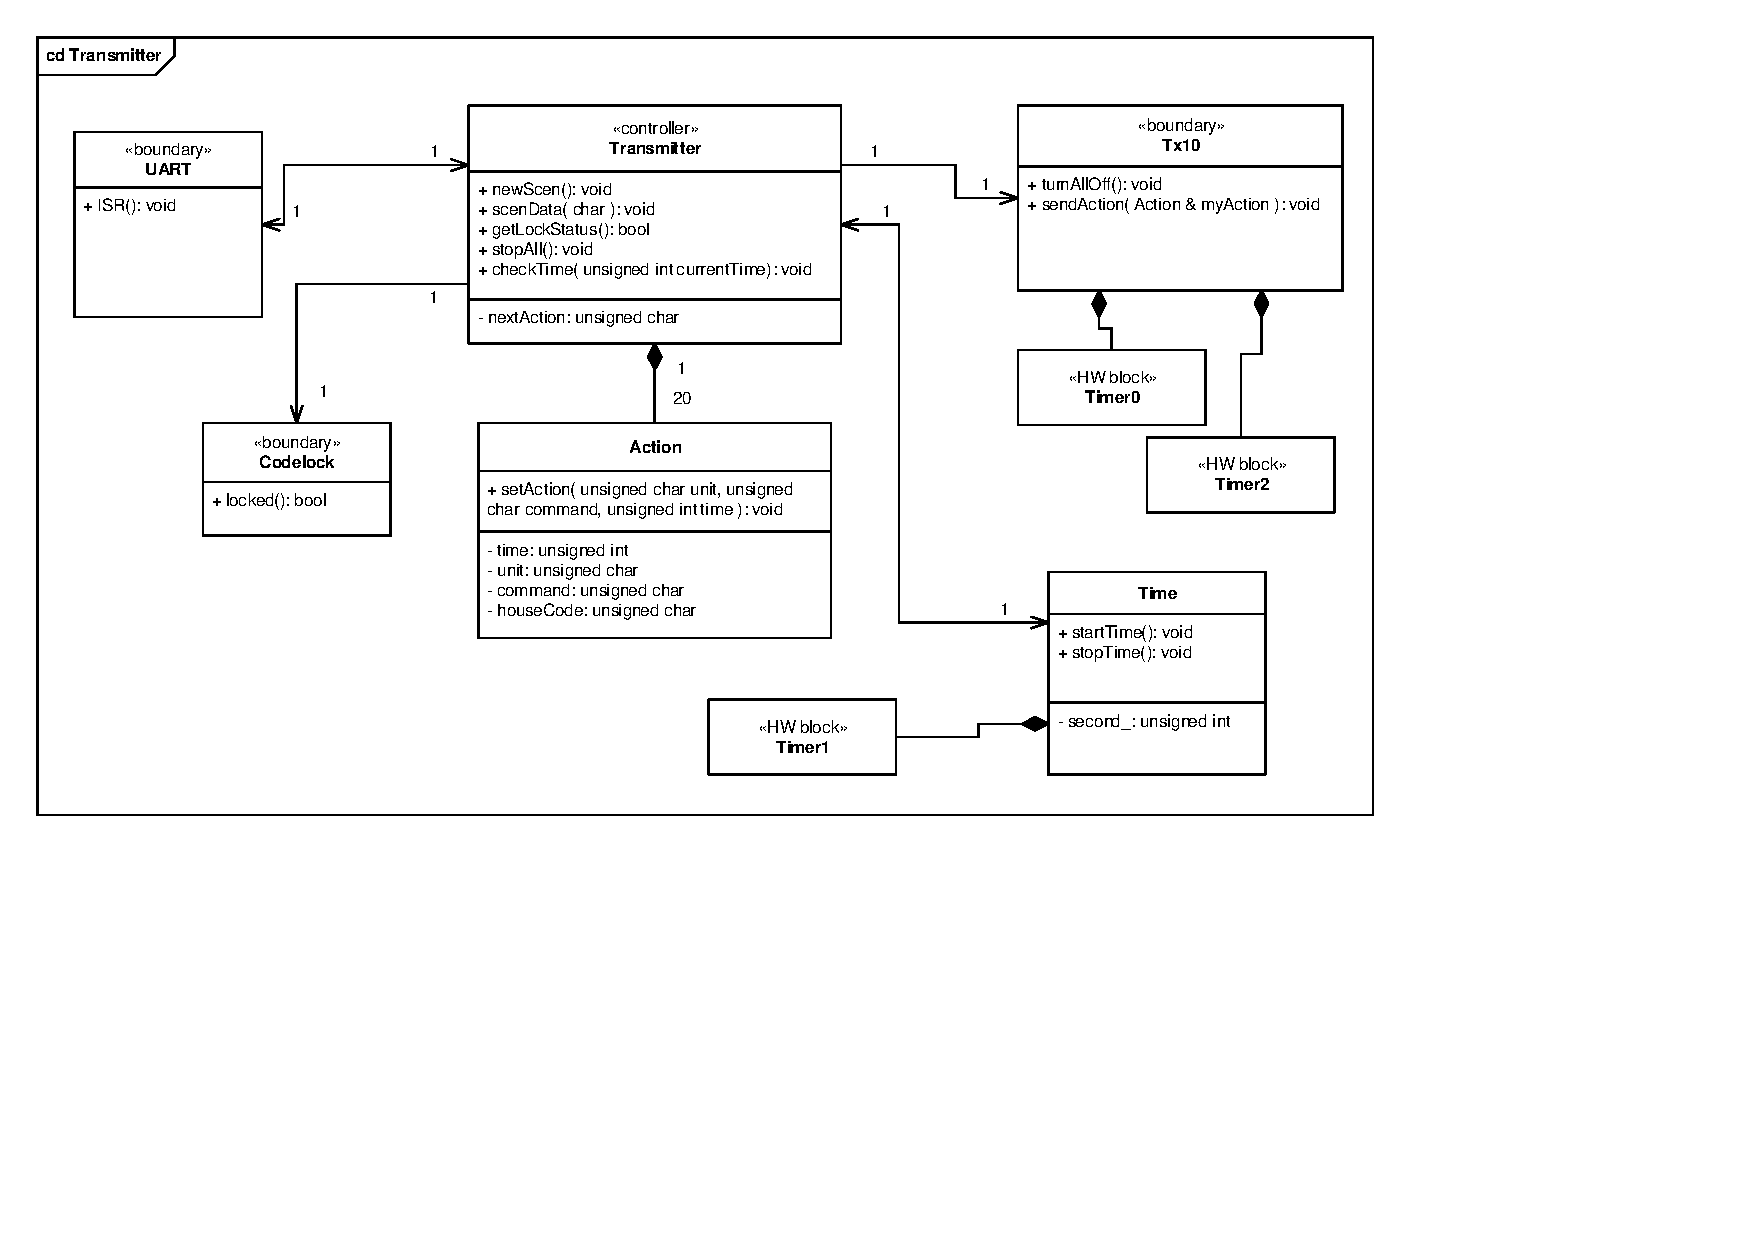
\includegraphics[scale=1,clip=true, trim=25 433 715 60]{Systemarkitektur/diagrammer/Transmitter_Klassediagram} %L B R T - HUSKE DET
\end{figure}

\begin{table}[h]
\begin{tabularx}{\textwidth}{p{0.6 cm} l X} %\hline
\multicolumn{3}{l}{\textbf{constructor}}\\
& Operation: & %Skriv tekst herunder
\texttt{UART} 
\\ & Parametre: & %Skriv tekst herunder
-
\\ & Returværdi: & %Skriv tekst herunder
- 
\\ & Beskrivelse: & %Skriv tekst herunder
opsætter forbindelse på RX og TX til UART, sætter op til brug af interupt.
\\ \end{tabularx}
\end{table}

\clearpage

\begin{table}[h]
\begin{tabularx}{\textwidth}{p{0.6 cm} l X} %\hline
\multicolumn{3}{l}{\textbf{ISR}}\\
& Operation: & %Skriv tekst herunder
\texttt{ISR()} 
\\ & Parametre: & %Skriv tekst herunder
-
\\ & Returværdi: & %Skriv tekst herunder
- 
\\ & Beskrivelse: & %Skriv tekst herunder
Ved interupt på UARTen går transmitteren i 'read mode'. Hvis UART'en læser et L som første char, tjekkes Lockstatus på kodelåsen og returneres til PCen. Hvis et N læses går UARTEN i 'receiving mode' og begynder at aflæse data på reciever pinen. se ref. (state-machine transmitter UART), for lagring af modtagne data. Hvis S modtages sættes transmitteren til 'stop mode'.
\\ \end{tabularx}
\end{table}


\subsection{Tx10 (Kristian T.)}

\begin{figure}[h]
\centering
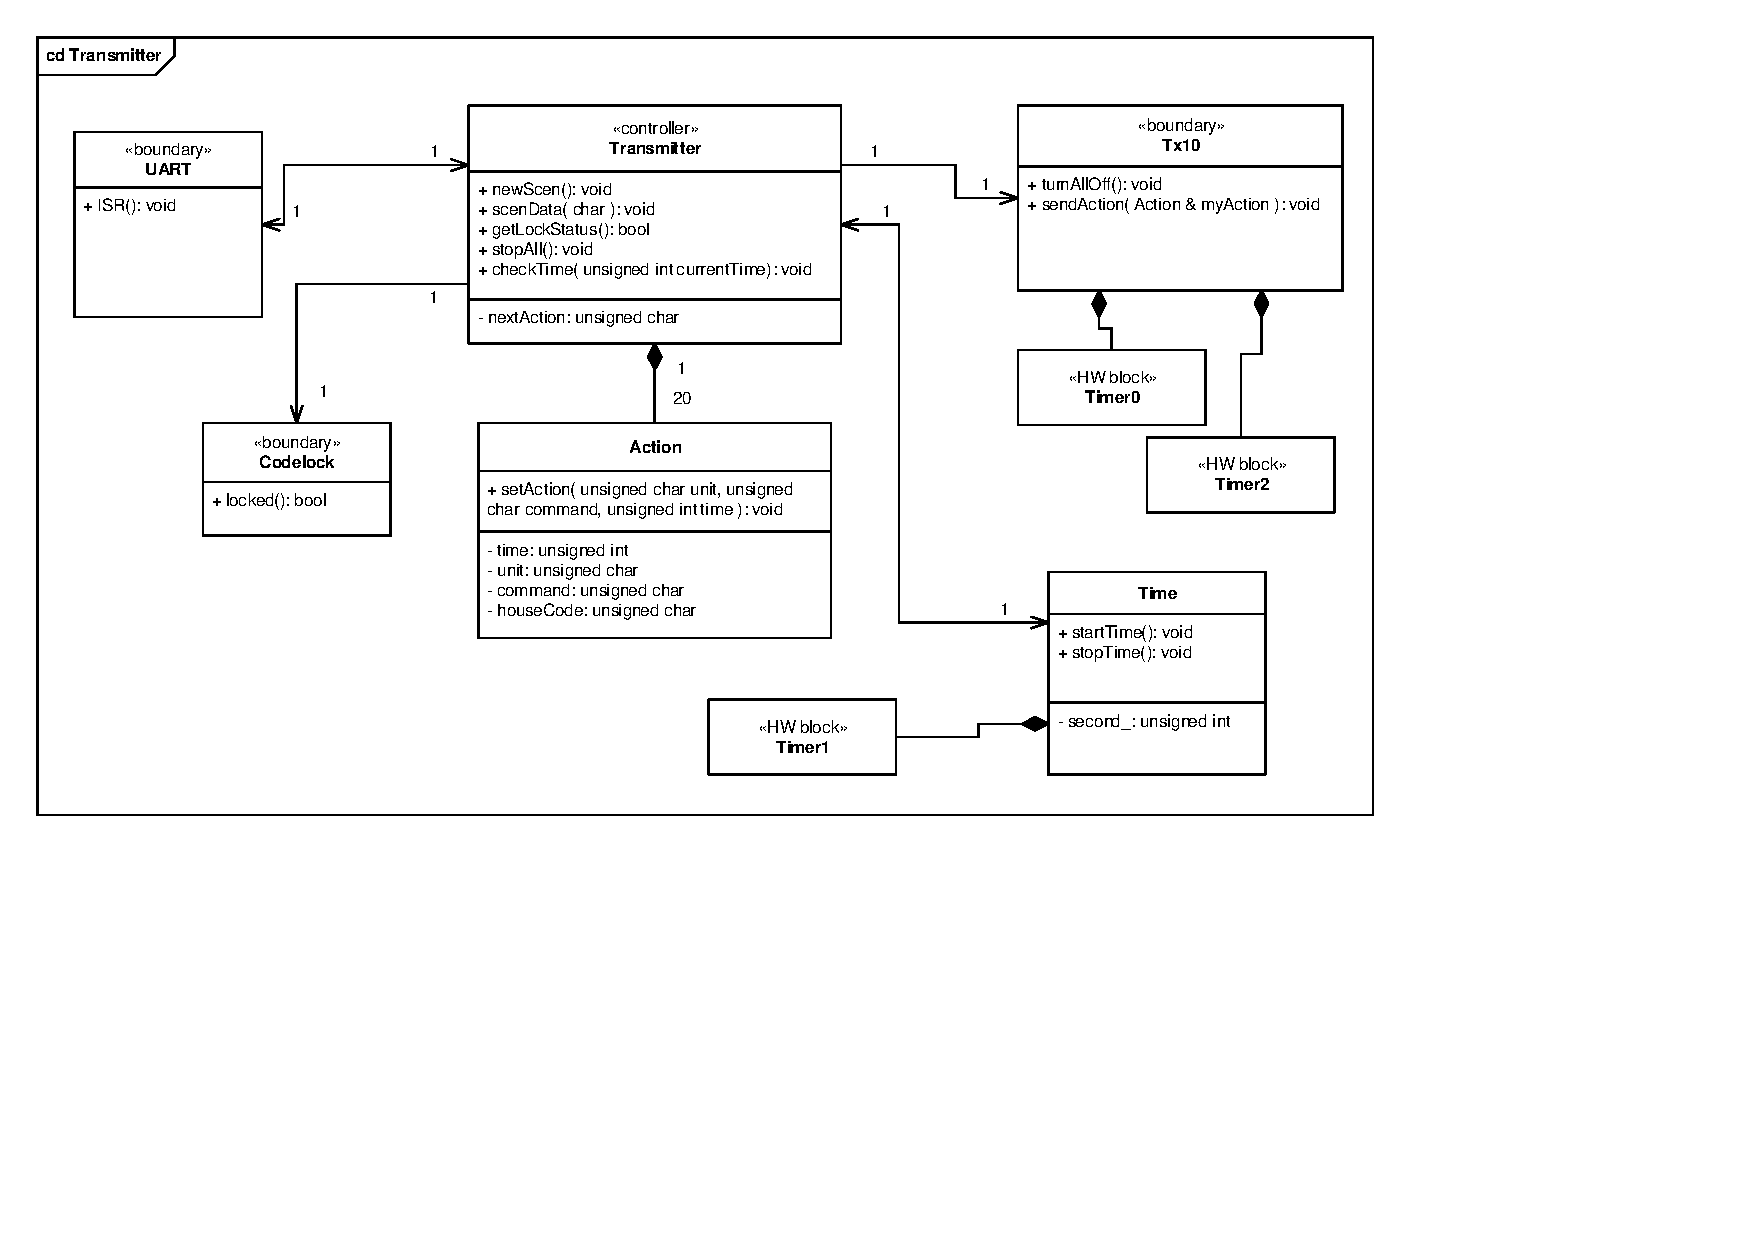
\includegraphics[scale=1,clip=true, trim=488.69 455 197 50]{Systemarkitektur/diagrammer/Transmitter_Klassediagram} %L B R T - HUSKE DET
\end{figure}

%turnAllOff
\begin{table}[h]
\begin{tabularx}{\textwidth}{p{0.6 cm} l X} %\hline
\multicolumn{3}{l}{\textbf{turnAllOff}}\\
& Operation: & %Skriv tekst herunder
\texttt{void turnAllOff()}
\\ & Parametre: & %Skriv tekst herunder
-
\\ & Returværdi: & %Skriv tekst herunder
-
\\ & Beskrivelse: & %Skriv tekst herunder
Når denne metode kaldes, sendes slukke-kommandoer ud til samtlige enheder på netværket via \texttt{sendAction()}.
\\ \end{tabularx}
\end{table}

%sendAction
\begin{table}[h]
\begin{tabularx}{\textwidth}{p{0.6 cm} l X} %\hline
\multicolumn{3}{l}{\textbf{sendAction}}\\
& Operation: & %Skriv tekst herunder
\texttt{void sendAction( Action \& myAction )} 
\\ & Parametre: & %Skriv tekst herunder
Modtager en reference til det pågældende objekt af klassen \texttt{Action}, som skal eksekveres.
\\ & Returværdi: & %Skriv tekst herunder
-
\\ & Beskrivelse: & %Skriv tekst herunder
Skal ved hjælp af protokollen for kommunikation over X.10 afsende kommandoer. Der skal sendes én bit hver anden interrupt/nulgennemgang på \texttt{PD2 (INT0)} (interrupt i toggle mode). Ved hver bit skal der ved det efterfølgende interrupt sendes det modsatte af det foregående. Hver gang et 1-tal skal sendes, skal dette være HIGH i 1 ms fra nulgennemgangen/interruptet.
\\ \end{tabularx}
\end{table}

\clearpage

%constructor
\begin{table}[h]
\begin{tabularx}{\textwidth}{p{0.6 cm} l X} %\hline
\multicolumn{3}{l}{\textbf{Constructor}}\\
& Operation: & %Skriv tekst herunder
\texttt{Tx10( void ) }
\\ & Parametre: & %Skriv tekst herunder
Ingen
\\ & Beskrivelse: & %Skriv tekst herunder
Skal initiere \texttt{Timer0} samt interrupt på \texttt{PD2 (INT0)}, men dog ikke aktivere disse.
\\ \end{tabularx}
\end{table}
